\documentclass[11pt,a4paper]{article}
\usepackage[utf8]{inputenc}
\usepackage[french]{babel}
\usepackage[T1]{fontenc}
\usepackage{amsmath, amssymb}
\usepackage{graphicx}
\usepackage{geometry}
\geometry{margin=1.5cm}
\usepackage{booktabs}
\usepackage{float}
\usepackage{caption}
\captionsetup{skip=3pt, font=small}

\title{Rapport scientifique sur l'innovation du groupe 3}
\author{Groupe 22 : Maxence RAYMOND || Nell TELECHEA-LOJOU}
\date{22 mai 2026}


\begin{document}

\maketitle

\section{Problème}

Le problème étudié consiste à maximiser la distance minimale entre un système de particules sur une trajectoire en losange.

\section{Critiques}

\subsection{Compréhension de l'article}

L'article est bien structuré et donne une réponse intéressante au problème. 
Cependant certains résultats sont surtout présentés de façon intuitive.
Le travail renvoit un effort d'organisation dans l'analyse, notamment dans la distinction des différents cas de configuration et dans la volonté de raisonner sur des propriétés de symétrie.
Le protocole expérimental permet de confronter les résultats théoriques aux observations issues des simulations.

\subsection{Analyse mathématique}

L'optimisation est une idée géométrique simple, ce qui rend la méthode facilement compréhensible.
L'égalité Eaigu=Eobtus est donnée comme condition d'équilibre et est illustrée par une figure, mais elle est surtout obtenue par une recherche numérique, sans montrer pourquoi elle serait unique ou optimale.
Ensuite, la condition de validité du modèle (w/h $\le$ $\sqrt{4/3}$ $\simeq$ 1.155) est donnée comme une limite du système, sans vraie explication de son origine.

\section{Reproductibilité des résultats de recherche}

\begin{figure} [ht!]
    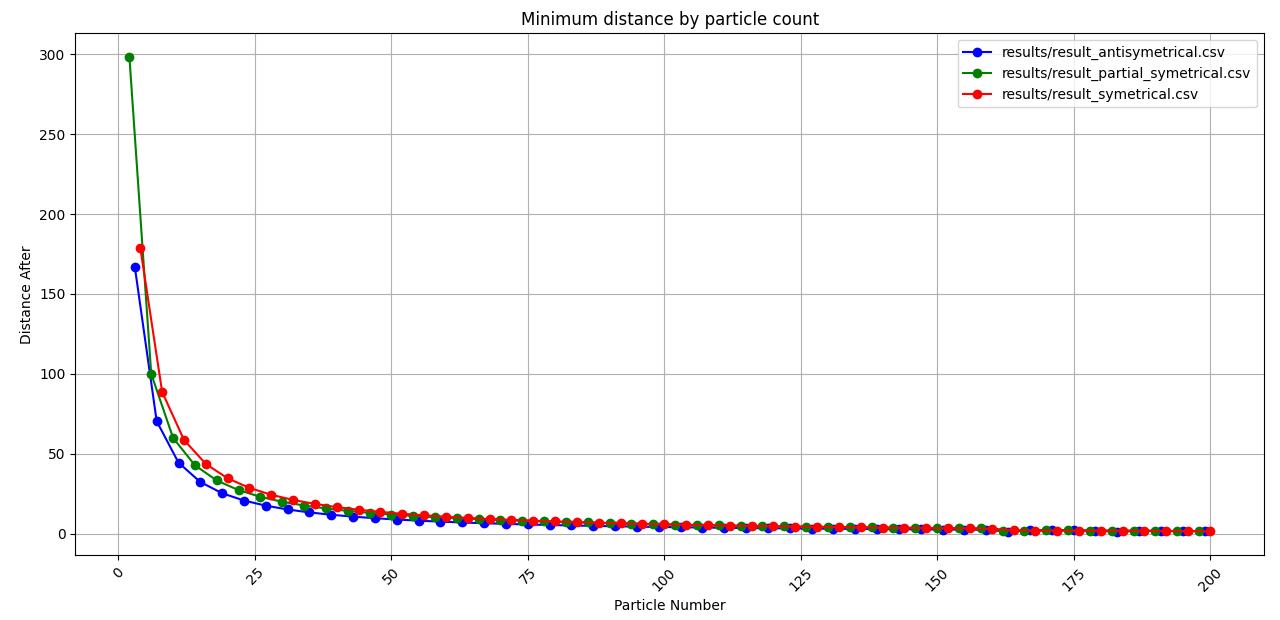
\includegraphics[width=\linewidth]{results/figure1.png}
    \caption{Figure 1 : Analyse graphique de la distance}	
\end{figure}

\begin{figure} [ht!]
    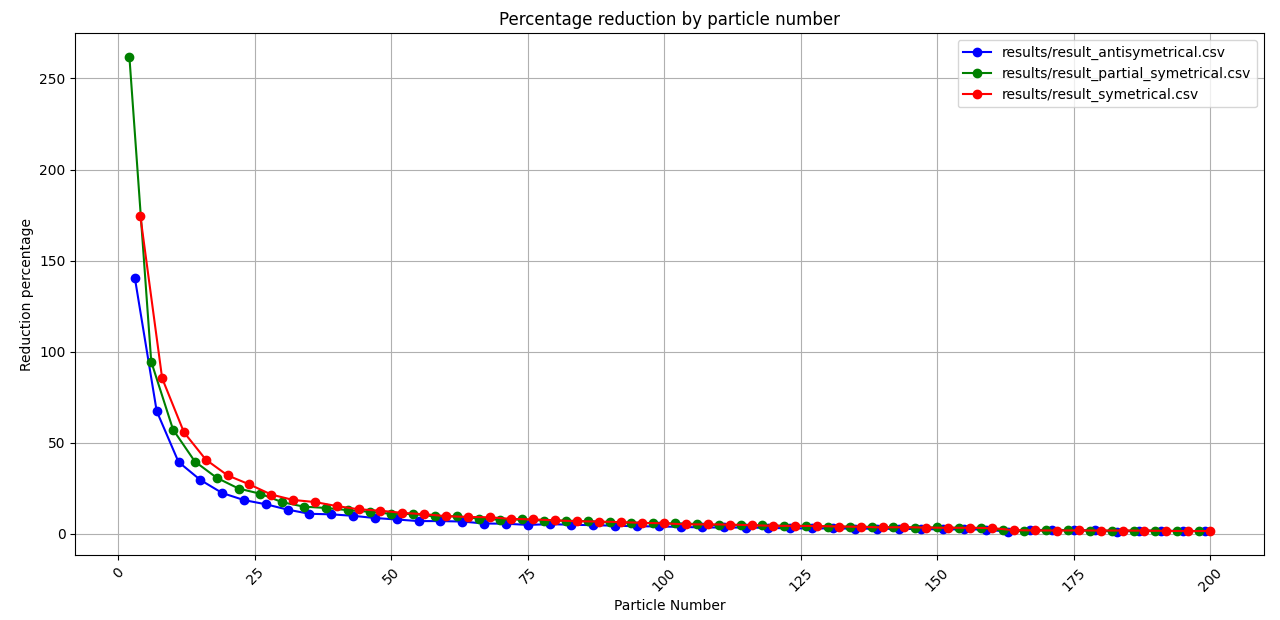
\includegraphics[width=\linewidth]{results/figure2.png}
    \caption{Figure 2 : Analyse graphique de l'amélioration}	
\end{figure}

\subsection{Code de l'innovation}

Le code de l'optimisation souffre de quelques défauts.
Parmi ces défauts, on peut retrouver des imports manquants dans le header et le fichier source, une fonction non standard utilisée qu'il a fallu recoder, ainsi qu'un manque de documentation sur l'argument T à passer à l'optimisation qui aurait été le bienvenu.

\subsection{Analyse des résultats}

\paragraph{Temps}

En effectuant les tests sur différents ordinateurs, on peut voir des résultats différents selon les ordinateurs.
Sur un ordinateur récent (processeur de douzième génération), le temps pris par l'algorithme est de moins d'un cycle de processseur de manière constante, correspondant au temps donné d'O(1).
Cependant, sur un ordinateur avec des capacités plus limitées (processeur de quatrième génération), le nombre de cycles utilisés croit avec le nombre de particules avec un ordre d'environ 0.09*n uù n est le nombre de particules.
Cette augmentation est répartie sur chaque cas et possède également des variations internes d'ordre important, restant également très rapide.
Le calcul de complexité algorithmique est plutôt de l'ordre de O(n+1), l'optimisation correspondant à une boucle et quelques calculs préalables.

\paragraph{Courbe}

La figure 1 représente une courbe suivant l'évolution de la distance minimale des particules pour chaque cas mentionné dans l'article. Elle a été générée à partir des fichiers csv générés par reproduction.c. 
Comme on peut le voir sur la figure 1, la distance minimale entre chaque point diminue de prévisible alors que le nombre de particules augmente. On peut également voir une légère instabilité apparaitre aux alentours de 150 particules. On peut également voir que les différents cas se conforment à ceux rapportés dans l'article.
On peut également voir sur la figure 2 que l'amélioration de la minimisation de la distance décroit fortement avec le nombre de particules, de 260\% de réduction dans le meilleur des cas jusqu'à environ 1,5\% lorsque l'on se rapproche du nombre de 200 particules. On peut également voir des variations apparaitre autour de 150 particules, dûs aux interactions entre particules.

\section{Conclusion}

Cette innovation démontre une efficacité optimale lorsqu'elle est appliquée à un nombre limité de particules. Cependant, son utilité diminue à mesure que le nombre de particules augmente pour une taille donnée. En effet, plus la taille du système est importante, plus l'espace intersticiel entre les particules peut devenir significatif et donc donner de meilleurs résultats.
Les résultats obtenus confirment ainsi ceux rapportés dans l'article de référence.

\end{document}